\chapter{Bibliographic research}
\label{ch:research}

% https://www.ericsson.com/en/reports-and-papers/white-papers/drones-and-networks-ensuring-safe-and-secure-operations
% https://web.stanford.edu/class/cs231a/prev_projects_2016/deep-drone-object__2_.pdf

\section{Remote Drone Control}
\label{sec:research-remote-drone-control}
The article ~\cite{ericsson1} also approaches the topic of drone control. \
According ot it, most current drone use cases cover the situation in which the drone \
operator is in line of sight of the drone and has full control over it, with autonomous \
drones operating outside line of sight gaining more and more importance today. \
However, in the future the most common drone use cases will be the ones in which the drone \
operates autonomously outside line of sight ir without supervision.

\begin{figure}[ht]
    \label{fig:drone-uses}
    %\centering
    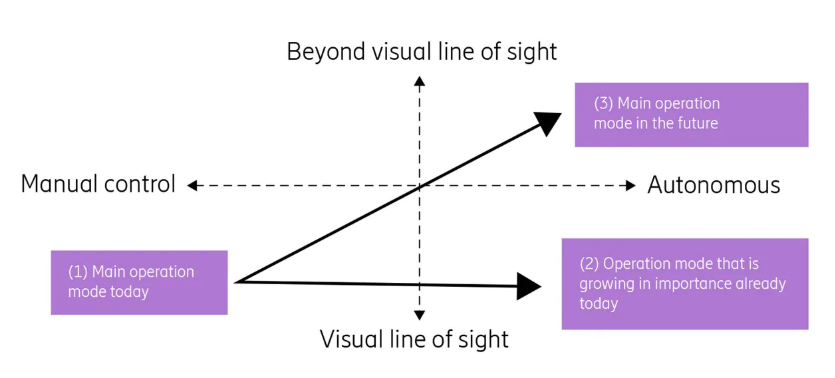
\includegraphics[width=15cm, height=50cm,keepaspectratio]{img/drone_uses.png}
    \caption{Drone Uses according to ~\cite{ericsson1}}
\end{figure}

In ~\cite{ericsson1} mentions three different options for drone communication and control:
\begin{enumerate}
    \item \textbf{satellite technology} is currently in use today for some drones; \
            its drawbacks include high latency and costs and low throughput
    \item \textbf{dedicated drone terrestrial network} its drawbacks also include high \
            costs and the time it would take to setup an adequate coverage for drones
    \item \textbf{existing terrestrial mobile networks} they have low latency and costs and \
            high throughput; \
            additionally, they have also proven to be secure and robust
\end{enumerate}

Additionally, other requirements can be accomplished using 4G LTE and 5G features. \
For instance, drone tracking can be implemented using the mobile positioning service and \
could be queried from the mobile network.

Drone control is also mentioned in ~\cite{forbes1} . \
The article also mentions 2 possible control methods that are actively used and that \
partially overlap over those mentioned above. \
These are:
\begin{enumerate}
    \item \textbf{radio waves} these have limited range (an example of 100 miles is given);
    \item \textbf{satellite uplink} it takes footage an average 1.2-second delay to go from \
            a drone in Afghanistan to the operator in Virginia
\end{enumerate}

~\cite{forbes1} also does a classification of drones according to how they are commanded. \
Three classes of drones emerge:
\begin{enumerate}
    \item \textbf{remotely piloted} an operator has full control, while the drone can do \
            minimal actions by its own, like avoid crashing
    \item \textbf{semi-autonomous} the drone can perform all or some missions without any \
            human interaction, however an operator exists that can take over control at \
            any time
    \item \textbf{fully autonomous} the drone is engineered to accomplish its mission \
            without any human interaction or supervision; \
            the command link can be missing
\end{enumerate}

\section{Object Detection}
\label{sec:research-object-detection}
In recent years, convolutional neural networks have been used more and more in \
the field of object detection. \
According to ~\cite{deepLearning}, A convolutional neural network (CNN) is a \
subclass of multilayer neural networks in which at least one layer applies \
a convolution on its input data instead of matrix multiplication.\
CNNs have seen a rise in use in object detection since 2012, when \
a CNN developed by ~\cite{imagenet} won the ImageNet Large Scale Visual \
Recognition Challenge for the first time. \
The CNN managed to reduce the top-1 (actual label differs from predicted label) \
 and top-5 (actual label is not in the predicted top 5 most likely labels) \
error rates from 47.1\% respectively 28.2\% to 37.5\% respectively 17\%. \
Additionally, the authors mentioned that the performance was limited by the \
existing hardware and dataset
Ever since, the contest has been won by convolutional neural networks. \
By 2016, the top-5 error rate dropped to 3.6\%.

In the paper~\cite{deepDrone}, the authors also attempt to create a drone capable \
of detecting people, with a few differences:
\begin{itemize}
    \item the drone is an airborne one
    \item image processing is done on the drone itself
\end{itemize}

% todo: mention SSD vs YOLO








%Bibliographic research has as an objective the establishment of the references for the \
%project, within the project domain/thematic. While writing this chapter (in general the \
%whole document), the author will consider the knowledge accumulated from several \
%dedicated disciplines in the second semester, 4$^{th}$ year (Project Elaboration \
%Methodology, etc.), and other disciplines that are relevant to the project theme.
%
%Represents about 15\% of the paper.
%
%Each reference must be cited within the document text, see example below (depending \
%on the project theme, the presentation of a method/application can vary).
%
%
%This section includes citations for conferences or workshop~\cite{BellucciLZ04}, \
%journals~\cite{AntoniouSBDB07},
%and books~\cite{russell1995artificial}.
%
%In paper~\cite{AntoniouSBDB07} the authors present a detection system for moving obstacles based on stereovision and ego motion estimation.
%The method is ... {\it discus the algorithms, data structures, functionality, specific aspects related to the project theme, etc.}... Discussion: {\it pros and cons}.
%
%In chapter~\ref{ch:analysis} of~\cite{strunk}, the {\it similar-to-my-project-theme algorithm} is presented, with the following features ...
%
%
%\section{Title}
%\section{Other title}
